%----------------------------------------------------------------------------------------
%	PACKAGES AND THEMES
%----------------------------------------------------------------------------------------

\documentclass{beamer}
\usepackage{ragged2e}
\justifying

\mode<presentation> {
\usetheme{CambridgeUS}
\usecolortheme{dolphin}
\setbeamertemplate{navigation symbols}{}}

\usepackage[utf8]{inputenc}
\usepackage[T1]{fontenc}
\usepackage[british]{babel}
\usepackage{amsmath,amsthm,amssymb,amsfonts}
\usepackage{enumerate}
\newcommand{\bm}{\boldsymbol}
\newcommand{\ds}{\displaystyle}
\newcommand{\mA}{{\mathbb A}}
\newcommand{\mB}{{\mathbb B}}
\newcommand{\mC}{{\mathbb C}}
\newcommand{\mD}{{\mathbb D}}
\newcommand{\mE}{{\mathbb E}}
\newcommand{\mI}{{\mathbb I}}
\newcommand{\mN}{{\mathbb N}}
\newcommand{\mQ}{{\mathbb Q}}
\newcommand{\mP}{{\mathbb P}}
\newcommand{\mR}{{\mathbb R}}
\newcommand{\mS}{{\mathbb S}}
\newcommand{\mZ}{{\mathbb Z}}
\newcommand{\cA}{{\mathcal A}}
\newcommand{\cb}{{\mathcal B}}
\newcommand{\cC}{{\mathcal C}}
\newcommand{\cE}{{\mathcal E}}
\newcommand{\cF}{{\mathcal F}}
\newcommand{\cG}{{\mathcal G}}
\newcommand{\cH}{{\mathcal H}}
\newcommand{\cI}{{\mathcal I}}
\newcommand{\cJ}{{\mathcal J}}
\newcommand{\cL}{{\mathcal L}}
\newcommand{\cM}{{\mathcal M}}
\newcommand{\cO}{{\mathcal O}}
\newcommand{\cP}{{\mathcal P}}
\newcommand{\cT}{{\mathcal T}}
\newcommand{\cU}{{\mathcal U}}
\newcommand{\cV}{{\mathcal V}}
\newcommand{\cZ}{{\mathcal Z}}
\newcommand{\sM}{{\mathscr M}}
\newcommand*{\defeq}{\mathrel{\vcenter{\baselineskip0.5ex \lineskiplimit0pt
                     \hbox{\scriptsize.}\hbox{\scriptsize.}}}%
                     =}
\usepackage{mathrsfs}

\usepackage[version=3]{mhchem}

\newcommand{\quotes}[1]{``#1''}

%----------------------------------------------------------------------------------------
% GRAPHICS
%----------------------------------------------------------------------------------------

\usepackage{graphicx}
\usepackage{tikz}
\usepackage{epstopdf}
\usepackage{color}
\definecolor{mygreen}{rgb}{0,0.6,0}
\definecolor{myred}{RGB}{139,0,0}
\definecolor{myblue}{RGB}{0,0,205}
\definecolor{myorange}{RGB}{255,140,0}
\usepackage{booktabs} % Allows the use of \toprule, \midrule and \bottomrule in tables

%----------------------------------------------------------------------------------------
%	TITLE PAGE
%----------------------------------------------------------------------------------------

\title[Combustion of rocket propellant]{Equilibrium for combustion of rocket propellant}
\author[Team Rocket]{A. Delgado, F. Granell, M. Llin\`as and J. Puig}
\institute[MMT]{Mathematical Models of Technology}
\date{Wednesday, 4th Oct 2015}

\begin{document}

\begin{frame}
\titlepage
\end{frame}

\begin{frame}
\frametitle{Overview}
\tableofcontents
\end{frame}

%----------------------------------------------------------------------------------------
%	PRESENTATION SLIDES
%----------------------------------------------------------------------------------------

\section{Statement of the problem}

%------------------------------------------------

\begin{frame}
\frametitle{Motivation}
\begin{itemize}
\item Reactions of combustion at high temperatures.
\item Dissociation of species.
\item Examples: propulsion of rockets.
\item Provide a solver for combustion of gas mixtures.
\end{itemize}
\end{frame}

%------------------------------------------------

\begin{frame}
\frametitle{How does a rocket work?}
\begin{figure}
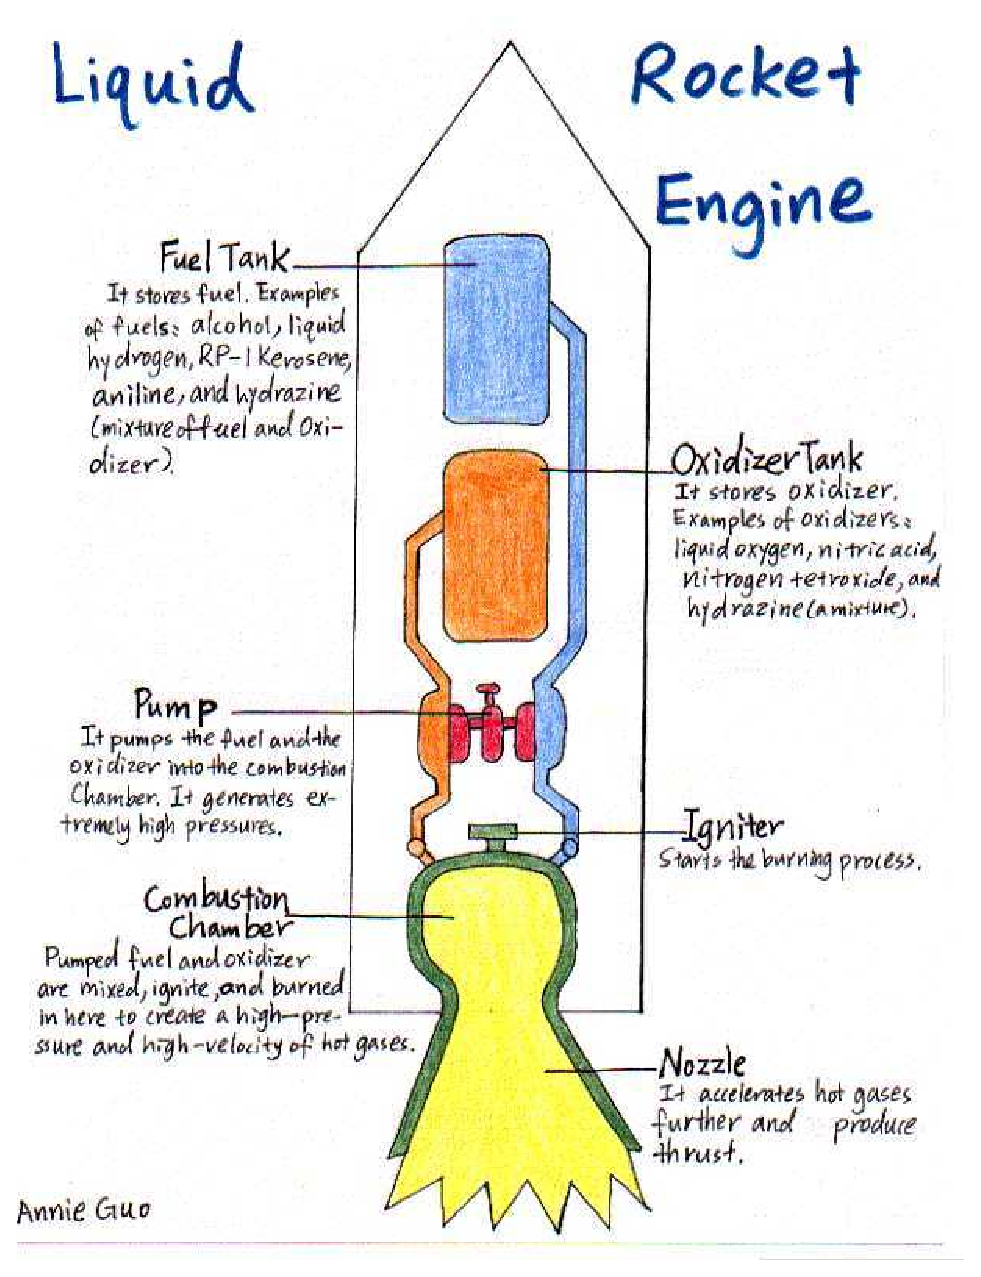
\includegraphics[width=0.5\linewidth]{rocket}
\end{figure}
\end{frame}

\section{Preliminary concepts}

%------------------------------------------------

\subsection{Review of Kinetic Molecular Theory}

%------------------------------------------------

\begin{frame}
\frametitle{How gases behave I}
\begin{block}{Ideal gases}
Given the pressure $P$, volume $V$ and temperature $T$ of an ideal gas,
\begin{equation*}
PV=nRT, \ R=0,082 \text{ atm}\cdot\text{L}\cdot\text{mol}^{-1}\cdot\text{K}^{-1},
\end{equation*}
where $n$ is the number of moles contained in the gas. An equivalent expression is
\begin{equation*}
PM=\rho RT,
\end{equation*}
where $M$ is the molecular mass of the gas and $\rho$ is its density.
\end{block}
\end{frame}

%------------------------------------------------

\begin{frame}
\frametitle{How gases behave II}
\begin{block}{Dalton's Law of Partial Pressures}
The total pressure of a mixture of gases equals the sum of the partial pressures. Mathematically, given a mixture of $n$ gases in a container,
\begin{equation*}
P = \sum_{i = 1}^n P_i.
\end{equation*}
We can express the partial pressure of each component in the mixture as
\begin{equation*}
P_i = n_i\frac{RT}{V} = n_i\frac{P}{n} = \frac{n_i}{n}P = \chi_i P,
\end{equation*}
\end{block}
\end{frame}

%------------------------------------------------

\begin{frame}
\frametitle{How gases behave III}
\begin{block}{Molar fraction}
The molar fraction $\chi_i$ of the gas $i$ is
\begin{equation*}
\chi_i = \frac{n_i}{n} = \frac{P_i}{P} = \frac{V_i}{V}.
\end{equation*}
\end{block}
\end{frame}

%------------------------------------------------

\subsection{Review of Thermodynamics}

%------------------------------------------------

\begin{frame}
\frametitle{First Law of Thermodynamics}
The total energy of an isolated system is constant. Mathematically, we write
\begin{equation*}
\Delta U = Q + W,
\end{equation*}
where $U$ is the internal energy, $Q$ is the heat involved in the process and $W$ is the work performed through compression or expansion of the system, which can be written as
\begin{equation*}
W = -P_{\text{ext}}\Delta V = -\Delta nRT,
\end{equation*}
where $P_{\text{ext}}$ is the pressure that the exterior exerts upon the gas and $\Delta n$ is the variation in the number of moles.
\end{frame}

%------------------------------------------------

\begin{frame}
\frametitle{Constant-volume and constant-pressure reactions}
If a reaction occurs at a constant volume, there is no work performed. Hence,
\begin{equation*}
\Delta U = Q_v,
\end{equation*}
where the constant-volume heat can be written as  $ Q_v = Q_p + W$.
\begin{block}{Enthalpy}
Let us define the \textit{enthalpy} $H$ as
\begin{equation*}
H = U + PV.
\end{equation*}
Indeed, in constant-pressure systems we can write
\begin{equation*}
\Delta H = (U_f + PV_f) - (U_i + PV_i) = \Delta U + P\Delta V,
\end{equation*}
and so $\Delta H = Q_p$.
\end{block}
It is important to notice that enthalpy is a thermodynamic potential
\end{frame}

%------------------------------------------------

\begin{frame}
\frametitle{Enthalpies of reaction}
\begin{block}{Standard enthalpy of reaction}
The standard enthalpy of reaction $\Delta H_r^0$ is the change in the enthalpy of a reaction in which the reagents and products are at standard conditions of pressure and temperature (if not stated differently).
\end{block}
\begin{block}{Standard enthalpy of formation}
The standard enthalpy of formation $\Delta H_f^0$ corresponds to the formation of 1 mol of a substance from the basic elements in the standard states of reference.
\end{block}
Other particular cases are
\begin{itemize}
\item reticular energy
\item bond dissociation energy
\end{itemize}
\end{frame}

%------------------------------------------------

\begin{frame}
\frametitle{Ways to calculate enthalpies}
\begin{block}{From enthalpies of formation}
The standard enthalpy of a reaction $\Delta H_r^0$ can be calculated using the formula
\begin{equation*}
\Delta H_r^0=\sum_{p\in P}v_p\Delta H_f^0(p) - \sum_{r\in R} v_r\Delta_f^0(r),
\end{equation*}
where $P$ and $R$ are the set of products and reagents, respectively, and $v_p$ and $v_r$ are the stoichiometric coefficients in the reaction.
\end{block}
\begin{block}{Hess's Law}
If a reaction can be expressed as the sum of several elementary reactions, then the variation in the enthalpy of the reaction can be calculated adding up the variations in the enthalpy of each elementary reaction.
\end{block}
\end{frame}

%------------------------------------------------

\begin{frame}
\frametitle{Enthalpy diagrams}
\begin{figure}
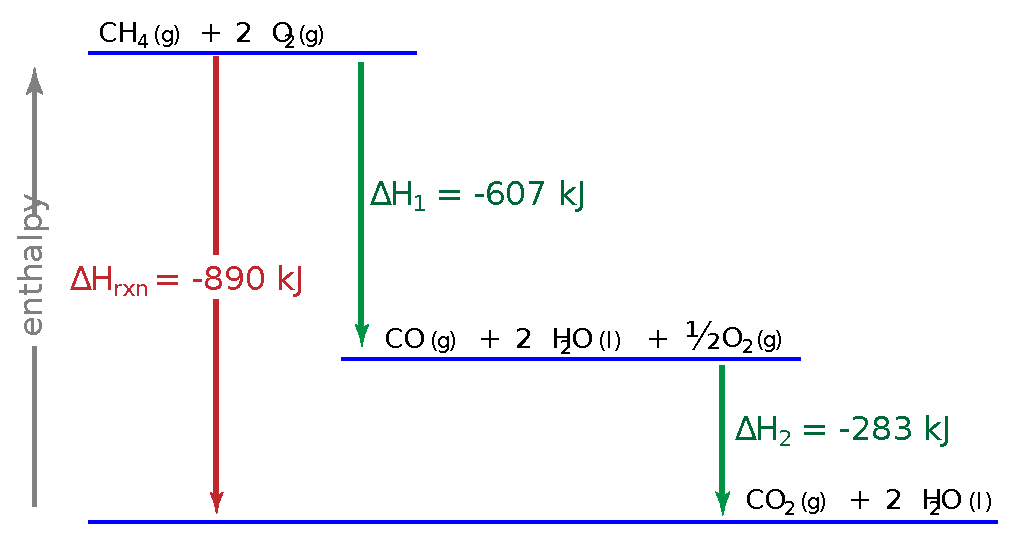
\includegraphics[width=0.9\linewidth]{hess-law}
\end{figure}
\end{frame}

%------------------------------------------------

\begin{frame}
\frametitle{Second and Third Laws of Thermodynamics}
\begin{block}{Second Law of Thermodynamics}
The entropy is a measure of disorder, and for an isolated system it never decreases, but grows until the thermodynamic equilibrium is attained. For a given system, the change in entropy can be expressed as
\begin{equation*}
\Delta S = \frac{Q_{\text{rev}}}{T},
\end{equation*}
where $Q_{\text{rev}}$ is the reversible heat or heat that intervenes in a reversible process.
\end{block}
\begin{block}{Third Law of Thermodynamics}
The entropy of a perfect pure crystal at 0 K is zero.
\end{block}
\end{frame}

%------------------------------------------------

\begin{frame}
\frametitle{Spontaneity} 
We can assume that the variation in the entropy of the environment is due to $-\Delta H_{\text{system}}$. Hence,
\begin{equation*}
0<\Delta S_{\text{universe}} = \Delta S_{\text{system}} + \Delta S_{\text{environment}}=\Delta S_{\text{system}}-\frac{\Delta H_{\text{system}}}{T},
\end{equation*}
so $\Delta H_{\text{system}} - T\Delta S < 0$.
\begin{block}{Gibbs free energy}
G = H - TS.
\end{block}
\begin{block}{Criteria for predicting the nature of a thermodynamic process.}
\begin{table}[h]
\begin{center}
\begin{tabular}{cccc}
   $\Delta H$ & $\Delta S$ & $\Delta G$ & Nature of the process  \\ \hline
   $-$ & $-$ & ? & spontaneous for small $T$\\
   $-$ & $+$ & $-$ & spontaneous\\
   $+$ & $+$ & ? & spontaneous for large $T$\\
   $+$ & $-$ & $+$ & non spontaneous\\
\end{tabular}
\end{center}
\end{table}
\end{block}
\end{frame}

%------------------------------------------------

\subsection{Review of Chemical Equilibrium}

%------------------------------------------------

\begin{frame}
\frametitle{Chemical equilibrium I}
Chemical equilibrium is a state in which the species involved remain constant along time
\begin{block}{Law of Mass Action}
Given the reaction
\begin{center}
\ce{$a$A + $b$B + $\dots$ <=> $g$G + $h$H + $\dots$}
\end{center}
there exists a constant that depends on the temperature. It is called the equilibrium constant and is calculated as
\begin{equation*}
K_c = \frac{[G]^g\cdot [H]^h\cdot\dots}{[A]^a\cdot [B]^b\cdot\dots},
\end{equation*}
where $[X]$ is the concentration of the substance X.
\end{block}
\end{frame}

%------------------------------------------------

\begin{frame}
\frametitle{Chemical equilibrium II}
\begin{block}{Other equilibrium constants}
The constants
\begin{equation*}
K_P = \frac{P_G^g\cdot P_H^h\cdot\dots}{P_A^a\cdot P_B^b\cdot\dots},  \ K_\chi = \frac{\chi_G^g\cdot\chi_H^h\cdot\dots}{\chi_A^a\cdot \chi_B^b\cdot\dots}, \ \text{and} \ K_n = \frac{n_G^g\cdot n_H^h\cdot\dots}{n_A^a\cdot n_B^b\cdot\dots}
\end{equation*}
are related through the expressions
\begin{equation*}
K_P = K_c(RT)^{\Delta n} = K_n\left(\frac{RT}{V}\right)^{\Delta n} = K_\chi P^{\Delta n},
\end{equation*}
where $\Delta n= g + h + \dots - (a + b + \dots)$.
\end{block}
\end{frame}

%------------------------------------------------

\begin{frame}
\frametitle{Chemical equilibrium III}
\begin{block}{Relation between the constants of different reactions}
Let us denote by $r_1$ the reaction
\begin{center}
\ce{$a$A + $b$B + $\dots$ <=> $g$G + $h$H + $\dots$}
\end{center}
and by $r_2$ and $r_3$ the inverse reaction and the same reaction with stoichiometric coefficients multiplied by $k\in\mN$, respectively. If $r_4$ is the reaction consisting of $r_1$ and $r_3$ happening simultaneously, then their equilibrium constants are affected by
\begin{equation*}
K_{c_{2}} = K_c^{-1}, \qquad K_{c_{3}} = K_c^k, \qquad \text{and} \qquad K_{c_{4}} = K_c K_{c_{3}},
\end{equation*}
where $K_{c_i}$ is the equilibrium constant of the reaction $r_i$.
\end{block}
\end{frame}

%------------------------------------------------

\begin{frame}
\frametitle{Chemical equilibrium IV}
\begin{block}{Predicting which way a reaction goes}
Let us define the reaction quotient $Q_c$ as
\begin{equation*}
Q_c= \frac{[G]_0^g\cdot [H]_0^h\cdot\dots}{[A]_0^a\cdot [B]_0^b\cdot\dots},
\end{equation*}
where $[X]_0$ is the initial concentration of the substance X. Then, if $Q_c<K_c$, the reaction \quotes{goes to the right}, if $Q_c>K_c$, the reaction \quotes{goes to the left} and if $Q_c=K_c$, the reaction is in equilibrium.
\end{block}
\end{frame}

%------------------------------------------------

\section{Our approach to the problem}

%------------------------------------------------

\begin{frame}
\frametitle{Sketch of the procedure}
\begin{itemize}
\item Assume the only reagents are hydrogen and oxygen, through the species H$_2$, O$_2$, H$_2$O, H, O and OH$^-$. We would like to find which the reagents are.
\item There are infinitely many solutions and each one has an associated value for $G$.
\item We can formulate a minimisation convex problem for the Gibbs free energy.
\item The reaction that actually takes place is the one that has the minimum Gibbs free energy.
\end{itemize}
\end{frame}

%------------------------------------------------

\begin{frame}
\frametitle{Sketch of the procedure}
\begin{block}{Optimisation problem for the Gibbs free energy}
Let us consider the linear programming problem
\begin{equation*}
\left\{
\begin{array}{lcl}
\ds\min_{\bm x\in\mR^n} \Delta G = \Delta H-T\Delta S & &\text{objective function}\\
\text{s.t.} & A\bm x \leq \bm 0 & \text{constrictions}\\
& \bm l \leqslant \bm x \leqslant \bm u & \text{bounds}
\end{array}
\right.
\end{equation*}
\end{block}
\end{frame}

%------------------------------------------------
\section*{}

%------------------------------------------------

\begin{frame}
\Huge{\centerline{Thanks for your attention!!}}
\begin{figure}
\includegraphics[width=0.5\linewidth]{team-rocket}
\end{figure}
\end{frame}

%----------------------------------------------------------------------------------------

\end{document}